\documentclass[english,twoside, openright, hidelinks, 11 pt, class=report,crop=false]{standalone}
\usepackage[utf8]{inputenc}
\usepackage{lmodern} % load a font with all the characters
\usepackage{geometry}
\geometry{verbose,paperwidth=16 cm, paperheight=24 cm, inner=2.3cm, outer=1.7 cm, bmargin=2cm, tmargin=1.8cm}

\setlength{\parindent}{0bp}
\usepackage{import}
\usepackage[subpreambles=false]{standalone}
\usepackage{amsmath}
\usepackage{amssymb}
\usepackage{esint}
\usepackage{babel}
\usepackage{tabu}
\makeatother
\makeatletter

\usepackage{titlesec}
\usepackage{ragged2e}
\RaggedRight
\raggedbottom
\frenchspacing

\usepackage{graphicx}
\usepackage{float}
\usepackage{subfig}
\usepackage{placeins}
\usepackage{cancel}
\usepackage{framed}
\usepackage{wrapfig}
\usepackage[subfigure]{tocloft}
\usepackage[font=footnotesize,labelfont=sl]{caption} % Figure caption
\usepackage{bm}
\usepackage[dvipsnames, table]{xcolor}
\definecolor{shadecolor}{rgb}{0.105469, 0.613281, 1}
\definecolor{blue}{cmyk}{1, 0, 0, 0}
\definecolor{red}{cmyk}{0, 1, 1, 0}
\definecolor{green}{cmyk}{100,0,100,0}
\colorlet{shadecolor}{Emerald!15} 
\usepackage{icomma}
\makeatother
\usepackage[many]{tcolorbox}
\usepackage{multicol}
\usepackage{stackengine}
\usepackage{listings}
\usepackage{esvect} %For vectors with capital letters

% For tabular
\usepackage{array}
\usepackage{multirow}
\usepackage{longtable} %breakable table

% Ligningsreferanser
\usepackage{mathtools} % for mathclap

%\mathtoolsset{showonlyrefs}

% sections without numbering in toc
\newcommand\tsec[1]{\phantomsection \addcontentsline{toc}{section}{#1}
	\section*{#1}}

% index
\usepackage{imakeidx}
\makeindex[title=Indeks]

%Footnote:
\usepackage[bottom, hang, flushmargin]{footmisc}
\usepackage{perpage} 
\MakePerPage{footnote}
\addtolength{\footnotesep}{2mm}
\renewcommand{\thefootnote}{\arabic{footnote}}
\renewcommand\footnoterule{\rule{\linewidth}{0.4pt}}
\renewcommand{\thempfootnote}{\arabic{mpfootnote}}

%colors
\definecolor{c1}{cmyk}{0,0.5,1,0}
\definecolor{c2}{cmyk}{1,0.25,1,0}
\definecolor{n3}{cmyk}{1,0.,1,0}
\definecolor{neg}{cmyk}{1,0.,0.,0}


\newcommand{\nreq}[1]{
\begin{equation}
	#1
\end{equation}
}


% Equation comments
\newcommand{\cm}[1]{\llap{\coln{ #1}}}


\usepackage[inline]{enumitem}
\newcounter{rg}
\numberwithin{rg}{chapter}

\newcommand{\reg}[2][]{\begin{tcolorbox}[boxrule=0.3 mm,arc=0mm,colback=Blue!3] {\refstepcounter{rg}\phantomsection \large \textbf{\therg \;#1} \vspace{5 pt}}\newline #2  \end{tcolorbox} \vs}
\newcommand{\regdef}[2][]{\begin{tcolorbox}[boxrule=0.3 mm,arc=0mm,colback=Blue!3] {\refstepcounter{rg}\phantomsection \large \textbf{\therg \;#1} \vspace{5 pt}}\newline #2  \end{tcolorbox} \vs}
\newcommand{\words}[1]{\begin{tcolorbox}[boxrule=0.3 mm,arc=0mm,colback=Teal!3] #1  \end{tcolorbox} \vs}

\newcommand\alg[1]{\begin{align*} #1 \end{align*}}

\newcommand\eks[2][]{\begin{tcolorbox}[boxrule=0.3 mm,arc=0mm,enhanced jigsaw,breakable,colback=Green!5] {\large \textbf{\ekstitle #1} \vspace{5 pt}\\} #2 \end{tcolorbox}\vs}

\newcommand{\st}[1]{\begin{tcolorbox}[boxrule=0.0 mm,arc=0mm,enhanced jigsaw,breakable,colback=Yellow!7]{ #1} \end{tcolorbox}}

\newcommand{\spr}[1]{\begin{tcolorbox}[boxrule=0.3 mm,arc=0mm,enhanced jigsaw,breakable,colback=Yellow!7] {\large \textbf{\sprtitle} \vspace{5 pt}\\} #1 \end{tcolorbox}\vs}

\newcommand{\sym}[1]{\colorbox{NavyBlue!15}{#1}}

\newcommand{\info}[2]{\begin{tcolorbox}[boxrule=0.3 mm,arc=0mm,enhanced jigsaw,breakable,colback=Cyan!6] {\large \textbf{#1} \vspace{5 pt}\\} #2 \end{tcolorbox}
}

\newcommand\algv[1]{\vspace{-11 pt}\begin{align*} #1 \end{align*}}

\newcommand{\regv}{\vspace{5pt}}
\newcommand{\mer}{\textsl{\note}: }
\newcommand{\mers}[1]{{\footnotesize \mer #1}}
\newcommand\vsk{\vspace{11pt}}
\newcommand{\tbs}{\vspace{5pt}}
\newcommand\vs{\vspace{-11pt}}
\newcommand\vsb{\vspace{-16pt}}
\newcommand\vso{\vspace{-5pt}}
\newcommand\br{\\[5 pt]}
\newcommand{\figp}[1]{../fig/#1}
\newcommand\algvv[1]{\vs\vs\begin{align*} #1 \end{align*}}
\newcommand{\y}[1]{$ {#1} $}
\newcommand{\os}{\\[5 pt]}
\newcommand{\prbxl}[2]{
\parbox[l][][l]{#1\linewidth}{#2
	}}
\newcommand{\prbxr}[2]{\parbox[r][][l]{#1\linewidth}{
		\setlength{\abovedisplayskip}{5pt}
		\setlength{\belowdisplayskip}{5pt}	
		\setlength{\abovedisplayshortskip}{0pt}
		\setlength{\belowdisplayshortskip}{0pt} 
		\begin{shaded}
			\footnotesize	#2 \end{shaded}}}
\newcommand{\fgbxr}[2]{
	\parbox[r][][l]{#1\linewidth}{#2
}}		

\renewcommand{\cfttoctitlefont}{\Large\bfseries}
\setlength{\cftaftertoctitleskip}{0 pt}
\setlength{\cftbeforetoctitleskip}{0 pt}

\newcommand{\bs}{\\[3pt]}
\newcommand{\vn}{\\[6pt]}
\newcommand{\fig}[1]{\begin{figure}[H]
		\centering
		\includegraphics[]{\figp{#1}}
\end{figure}}

\newcommand{\localfig}[2]{\begin{figure}[H]
		\centering
		\includegraphics[scale=#2]{#1}
\end{figure}}

\newcommand{\figc}[2]{\begin{figure}
		\centering
		\includegraphics[]{\figp{#1}}
		\caption{#2}
\end{figure}}
\newcommand{\arc}[1]{{
		\setbox9=\hbox{#1}%
		\ooalign{\resizebox{\wd9}{\height}{\texttoptiebar{\phantom{A}}}\cr\textit{#1}}}}

\newcommand{\sectionbreak}{\clearpage} % New page on each section

\newcommand{\nn}[1]{
\begin{equation*}
	#1
\end{equation*}
}

\newcommand{\enh}[1]{\,\text{#1}}

%asin, atan, acos
\DeclareMathOperator{\atan}{atan}
\DeclareMathOperator{\acos}{acos}
\DeclareMathOperator{\asin}{asin}

% Comments % old cm, ggb cm is new
%\newcommand{\cm}[1]{\llap{\color{blue} #1}}

%%%

\newcommand\fork[2]{\begin{tcolorbox}[boxrule=0.3 mm,arc=0mm,enhanced jigsaw,breakable,colback=yellow!7] {\large \textbf{#1 (\expl)} \vspace{5 pt}\\} #2 \end{tcolorbox}\vspace{-5pt} }
 
%colors
\definecolor{projectgreen}{cmyk}{100,0,100,0}

\newcommand{\colr}[1]{{\color{Red} #1}}
\newcommand{\colb}[1]{{\color{Cyan} #1}}
\newcommand{\colo}[1]{{\color{Orange} #1}}
\newcommand{\colc}[1]{{\color{SeaGreen} #1}}
\newcommand{\colg}[1]{{\color{Green} #1}}
\newcommand{\coln}[1]{{\color{NavyBlue} #1}}

% Methods
\newcommand{\metode}[2]{
	\textsl{#1} \\ \vspace{-10pt}
	\rule{#2}{0.75pt}
}

%Opg
\newcommand{\abc}[1]{
	\begin{enumerate}[label=\alph*),leftmargin=18pt]
		#1
	\end{enumerate}
}
\newcommand{\abcs}[2]{
	\begin{enumerate}[label=\alph*),start=#1,leftmargin=18pt]
		#2
	\end{enumerate}
}
\newcommand{\abcn}[1]{
	\begin{enumerate}[label=\arabic*),leftmargin=18pt]
		#1
	\end{enumerate}
}




\newcommand{\abch}[1]{
	\hspace{-2pt}	\begin{enumerate*}[label=\alph*), itemjoin=\hspace{1cm}]
		#1
	\end{enumerate*}
}

\newcommand{\abchs}[2]{
	\hspace{-2pt}	\begin{enumerate*}[label=\alph*), itemjoin=\hspace{1cm}, start=#1]
		#2
	\end{enumerate*}
}

% Exercises


\newcounter{opg}
\numberwithin{opg}{section}

\newcounter{grub}
\numberwithin{opg}{section}
\newcommand{\op}[1]{\vspace{15pt} \refstepcounter{opg}\large \textbf{\color{NavyBlue}\theopg} \vspace{2 pt} \label{#1} \\}
\newcommand{\opd}[1]{\vspace{15pt} \refstepcounter{opg}\large \textbf{\color{NavyBlue}\theopg} 
\includegraphics{../../calculatorimage} \vspace{2 pt} \label{#1} \\}
\newcommand{\eksop}[2]{\vspace{15pt} \refstepcounter{opg}\large \textbf{\color{NavyBlue}\theopg} (#1) \vspace{2 pt} \label{#2} \\}

\newcommand{\nes}{\stepcounter{section}
	\setcounter{opg}{0}}
\newcommand{\opr}[1]{\vspace{3pt}\textbf{\ref{#1}}}
\newcommand{\oeks}[1]{\begin{tcolorbox}[boxrule=0.3 mm,arc=0mm,colback=white]
		\textit{\ekstitle: } #1	  
\end{tcolorbox}}
\newcommand\opgeks[2][]{\begin{tcolorbox}[boxrule=0.1 mm,arc=0mm,enhanced jigsaw,breakable,colback=white] {\footnotesize \textbf{\ekstitle #1} \\} \footnotesize #2 \end{tcolorbox}\vspace{-5pt} }


% tag exercises
\newcommand{\tagop}[1]{ 
{\small \color{Gray} #1} \os
}

% License
\newcommand{\lic}{
This book is part of the \net{https://sindrsh.github.io/openmathbooks/}{OpenMathBooks} project. OpenMathBooks © 2022 by Sindre Sogge Heggen is licensed under CC BY-NC-SA 4.0. To view a copy of this license, visit \net{http://creativecommons.org/licenses/by-nc-sa/4.0/}{http://creativecommons.org/licenses/by-nc-sa/4.0/}}

%referances
\newcommand{\net}[2]{{\color{NavyBlue}\href{#1}{#2}}}
\newcommand{\hrs}[2]{\hyperref[#1]{\color{NavyBlue}#2 \ref*{#1}}}
\newcommand{\refunnbr}[2]{\hyperref[#1]{\color{NavyBlue}#2}}


\newcommand{\openmath}{\net{https://sindrsh.github.io/openmathbooks/}{OpenMathBooks}}
\newcommand{\am}{\net{https://openmath.online/books/pdf/AM_bm.pdf}{AM1}}
\newcommand{\mb}{\net{https://openmath.online/books/pdf/MB_bm.pdf}{MB}}
\newcommand{\tmen}{\net{https://openmath.online/books/pdf/TM1_bm.pdf}{TM1}}
\newcommand{\tmto}{\net{https://openmath.online/books/pdf/TM2_bm.pdf}{TM2}}
\newcommand{\amto}{\net{https://sindrsh.github.io/FirstPrinciplesOfMath/}{AM2}}
\newcommand{\eksbm}{
\footnotesize
Dette er opppgaver som har blitt gitt ved sentralt utformet eksamen i Norge. Oppgavene er laget av Utdanningsdirektoratet. Forkortelser i parantes viser til følgende:
\begin{center}
	\begin{tabular}{c|c}
		E & Eksempeloppgave \\
		V/H & Eksamen fra vårsemesteret/høstsemesteret\\
		G/1P/1T/R1/R2 & Fag  \\
		XX & År 20XX \\
		D1/D2 & Del 1/Del 2
	\end{tabular}
\end{center}
Tekst og innhold kan her være noe endret i forhold til originalen.
}

%Excel og GGB:

\newcommand{\g}[1]{\begin{center} {\tt #1} \end{center}}
\newcommand{\gv}[1]{\begin{center} \vspace{-11 pt} {\tt #1}  \end{center}}
\newcommand{\cmds}[2]{{\tt #1}\\
	#2}

% outline word
\definecolor{Teal}{cmyk}{1, 0, 0.4, 0.3}
\newcommand{\outl}[1]{{\boldmath \color{Teal}\textbf{#1}}}
%line to seperate examples
\newcommand{\linje}{\rule{\linewidth}{1pt} }


%Vedlegg
\newcounter{vedl}
\newcounter{vedleq}
\renewcommand\thevedl{\Alph{vedl}}	
\newcommand{\nreqvd}{\refstepcounter{vedleq}\tag{\thevedl \thevedleq}}

%%% Writing code

\definecolor{codegreen}{rgb}{0,0.6,0}
\definecolor{codegray}{rgb}{0.5,0.5,0.5}
\definecolor{codepurple}{rgb}{0.58,0,0.82}
\definecolor{backcolour}{rgb}{0.95,0.95,0.92}


\lstdefinestyle{mystyle}{
	backgroundcolor=\color{backcolour},   
	commentstyle=\color{codegreen},
	keywordstyle=\color{magenta},
	numberstyle=\tiny\color{codegray},
	stringstyle=\color{codepurple},
	basicstyle=\ttfamily\footnotesize,
	breakatwhitespace=false,         
	breaklines=true,                 
	captionpos=b,                    
	keepspaces=true,                 
	numbers=left,                    
	numbersep=5pt,                  
	showspaces=false,                
	showstringspaces=false,
	showtabs=false,                  
	tabsize=2
}

\lstset{literate=%
	{æ}{{\ae}}1
	{ø}{{\o}}1
	{å}{{\aa}}1
}

\lstset{style=mystyle}


\newcommand{\pymet}[1]{{\ttfamily\color{magenta} #1}}
\newcommand{\pytype}[1]{{\ttfamily\color{codepurple} #1}}

\newcommand{\python}[1]{
\begin{tcolorbox}[boxrule=0.3 mm,arc=0mm,colback=white]
\lstinputlisting[language=Python]{#1}
\end{tcolorbox}}
\newcommand{\pythonut}[2]{
\begin{tcolorbox}[boxrule=0.3 mm,arc=0mm,colback=white]
\small 
%\textbf{Kode}
\lstinputlisting[language=Python]{#1}	
\vspace{11pt}
\textbf{Utdata} \\ \ttfamily
#2
\end{tcolorbox}}
%%%

%page number
%\usepackage{fancyhdr}
%\pagestyle{fancy}
%\fancyhf{}
%\renewcommand{\headrule}{}
%\fancyhead[RO, LE]{\thepage}

\newcommand{\deltax}{\,\text{d}x}
\newcommand{\deltau}{\,\text{d}u}
\usepackage{datetime2}
%%\usepackage{sansmathfonts} for dyslexia-friendly math
\usepackage[]{hyperref}

\newcommand{\texandasy}{Teksten er skrevet i \LaTeX\ og figurene er lagd ved hjelp av Asymptote.}

\newcommand{\expl}{forklaring}

\newcommand{\note}{Merk}
\newcommand{\notesm}[1]{{\footnotesize \textsl{\note:} #1}}
\newcommand{\ekstitle}{Eksempel }
\newcommand{\sprtitle}{Språkboksen}
\newcommand{\vedlegg}[1]{\section*{Vedlegg \thevedl: #1}  \setcounter{vedleq}{0} \refstepcounter{vedl}}

\newcommand\sv{\vsk \textbf{Svar} \vspace{4 pt}\\}

% exercises
\newcommand{\opgt}{\newpage \phantomsection \addcontentsline{toc}{section}{Oppgåver} \section*{Oppgaver for kapittel \thechapter}\vs \setcounter{section}{1}}

\newcommand{\grubop}[1]{\vspace{15pt} \refstepcounter{grub}\large \textbf{\color{NavyBlue} Gruble \thegrub} \vspace{2 pt} \label{#1} \\}
\newcommand{\grubeksop}[2]{\vspace{15pt} \refstepcounter{grub}\large \textbf{\color{NavyBlue} Gruble \thegrub} (#2) \vspace{2 pt} \label{#1} \\}
\newcommand{\gruboprecc}[1]{\vspace{15pt} \refstepcounter{grub}\large \textbf{\color{NavyBlue} Gruble* \thegrub} \vspace{2 pt} \label{#1} \\}
\newcommand{\grubeksoprecc}[2]{\vspace{15pt} \refstepcounter{grub}\large \textbf{\color{NavyBlue} Gruble* \thegrub} (#2) \vspace{2 pt} \label{#1} \\}
\newcommand{\grubr}[1]{\vspace{3pt}\textbf{Gruble \ref{#1}}}

%references
\newcommand{\reftab}[1]{\hrs{#1}{tabell}}
\newcommand{\rref}[1]{\hrs{#1}{regel}}
\newcommand{\dref}[1]{\hrs{#1}{definisjon}}
\newcommand{\refkap}[1]{\hrs{#1}{kapittel}}
\newcommand{\refsec}[1]{\hrs{#1}{seksjon}}
\newcommand{\refdsec}[1]{\hrs{#1}{delseksjon}}
\newcommand{\refved}[1]{\hrs{#1}{vedlegg}}
\newcommand{\eksref}[1]{\textsl{#1}}
\newcommand\fref[2][]{\hyperref[#2]{\textsl{figur \ref*{#2}#1}}}
\newcommand{\refop}[1]{{\color{blue}Oppgave \ref{#1}}}
\newcommand{\refops}[1]{{\color{blue}oppgave \ref{#1}}}

% Solutions manual
\newcommand{\selos}{Se løsningsforslag.}

\newcommand{\ompref}{Omgjøring av prefikser}


\begin{document}
%\setcounter{chapter}{4}	
	
\opgt



\eksop{GV26D1}{gv26d1opg2a}
En høyttaler er satt ned i pris fra 800\,kr til 640\,kr. Hvor stor er rabatten i prosent?

\eksop{1PH24D1}{1pH24d1opg1}
Prisen for en vare A øker fra 120 kroner til 180 kroner.\\
Prisen for en vare B øker fra 16 kroner til 26 kroner.\os

Hvilken pris øker prosentvis mest? Grunngi svaret.

\eksop{1PV23D1}{1pv23d1opg1}
Marko har kjøpt en sjokolade i enn butikk. Den kostet 20 kroner.
Mari har kjøp den samme sjokoladen på en bensinstasjon. Den kostet 50 kroner. \os

Avgjør om påstandene under er riktige. Grunngi svaret ditt. \os

\begin{tabular}{p{2cm} | p{10cm}}
	\hline
	Påstand 1 & ''Sjokoladen er
	150\% dyrere på bensinstasjonen enn i butikken.'' \\ \hline
	Påstand 2 & ''Sjokoladen er
	60\% billigere i butikken enn på bensinstasjonen.'' \\ \hline
\end{tabular}
 \os



\st{
\textbf{Konsumprisinder}\footnote{Hentet fra \net{https://www.ssb.no/priser-og-prisindekser/konsumpriser/statistikk/konsumprisindeksen}{ssb.no}.} \vsk

	
\parbox{0.25\linewidth}{	\begin{tabular}{c|c}
		År &  KPI \\ \hline
		2020 & 112,2\\
		2019 & 	110,8\\
		2018 &  112,2 \\
		2017&	105,5\\
		2016&	103,6\\
		2015&	100\\
		2014&	97,9\\
		2013&	95,9\\
		2012&	93,9\\
		2011&	93,3\\
		2010&	92.1\\
		2009&	89.9\\		
\end{tabular}}
\parbox{0.45\linewidth}{	\begin{tabular}{c|c}
		 &   \\ \hline
		2008&	88\\
		2007&	84.8\\
		2006&	84.2\\
		2005&	82.3\\
		2004&	81\\
		2003&	80.7\\
		2002&	78.7\\
		2001&	77.7\\
		2000&	75.5\\
		1999&	73.2\\
		1998&	71.5\\
		1997&	69.9
\end{tabular}}
}

\nes

\op{opgkr}
Regn ut kroneverdien i årene:\os
\textbf{a)} 1998\qquad \textbf{b)} 2014 \qquad \textbf{c)} 2017


\op{opgelsereal}
I 2017 tjente Else 490 000 kr, mens hun i 2012 tjente 410 000 kr. I
2017 var KPI $ = $ 105,5, mens i 2012 var KPI $ = $ 93,9. 
\abc{
\item Finn reallønnen til Else i 2017 og i 2012. 
\item I hvilket av disse årene hadde Else best råd?
}

\eksop{2PV22D1}{2pv22d1opg3}
Tabellen viser konsumprisindeksen (KPI) for årene 2015\,--\,2021:
\begin{center}
	\begin{tabular}{l | c | c | c| c| c|c|c }
		År & 2015 & 2016  & 2017 & 2018 & 2019  & 2020 & 2021 \\ \hline
		KPI & 100 & 103,6 & 105,5 & 108,4 & 110,8 & 112,2 & 116,1
	\end{tabular}
\end{center}
I 2015 hadde Elin en nominell lønn på 400\,000 kroner.\\
I 2021 hadde hun en nominell lønn på 460\,000 kroner.\os 
I hvilket av disse to årene hadde hun størst kjøpekraft?


\nes

\eksop{GV25D2}{gv25d2opg3}
Jonas vil spare 20 000 kroner han tjente på sommerjobben, og setter pengene i banken.
Han har laget en funksjon $f(x)$ som gir hvor mye penger han vil ha i banken om $x$ år:
\[ f(x) = 20000\cdot 1,04^x \]
\abc{
\item Forklar hva tallene 20\,000 og 1,04, og variabelen $x$ betyr i sparingen til Jonas.
\item Bruk funksjonen og finn ut hvor mange kroner Jonas har i banken etter 15 år.
}

\eksop{1PV21D2}{1pv26d2opg2}
En scooter koster 12\,000\,kr. Scooterens verdi avtar med 12\;\%\\ hvert år. Hva er scooterens verdi etter 6 år?

\op{opgser}
Fra en bank låner du 200\,000 kr med 2\% i årlig rente. Lånet skal betales tilbake som et serielån med 10 årlige terminbeløp. \os
\textbf{a)} Hva blir det årlige avdraget?\os
\textbf{b)} Hva er gjelden din etter at du har betalt sjette terminbeløp?\os
\textbf{c)} Hvor mye må du betale i renter det sjuende terminbeløpet?\os
\textbf{d)} Hvor stort blir det sjuende terminbeløpet?\os 

\op{opganu}
Fra en bank låner du 100\,000\,kr med 2\% årlig rente. Lånet skal betales tilbake som et annuitetslån over 15 år, og banken har da regnet ut at terminbeløpet blir 7\,783.\os

Regn ut avdrag og renter for det første terminbeløpet.

\op{opgserogan}
Hvilken av figurene skisserer et serielån og hvilken skisserer et annuitetslån? Forklar hvorfor.
\begin{figure}	\centering
	\subfloat[]{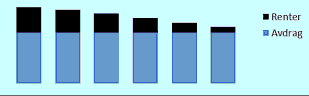
\includegraphics[scale=1]{ser}}\;
	\subfloat[]{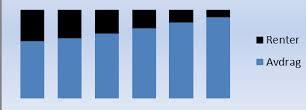
\includegraphics[scale=1]{an}}
\end{figure}

\op{opgspar}
Du oppretter en sparekonto i en bank som gir 2,3\% årlig rente og setter inn 45\,000\,kr. Hvor mye har du på kontoen etter 15 år?

\eksop{1PV22D1}{1PV22D1opg1}
Renten på et lån steg fra 2,0\% til 2,2\%.
\abc{
\item Hvor mange prosentpoeng steg renta med?
\item Hvor mange prosent steg renta med?
}
\newpage
\op{opgkred}
Tenk at kredittkortet ditt har 45 dagers lån uten renter, og 10\% månedlig rente etter dette. Du kjøper en scooter for 50\,000\,kr med kredittkortet. (Regn en måned som 30 dager.)\os
\textbf{a)} Hvor mye skylder du banken hvis ingenting er betalt innen 75 dager?\os
\textbf{b)} Hvor mye skylder du banken hvis ingenting er betalt innen 105 dager?\os 
\textbf{c)} Hvor mye skylder du banken etter 75 dager hvis du betalte 20\,000\,kr innen de første 45 dagene?



\nes

\op{opgpensj}
Børge har 350\,000\,kr i lønn. Børge er pensjonist, og skal da ha 56\,000\,kr i personfradrag og 83\,000\,kr i minstefradrag. I tillegg betaler han 700\,kr i fagforeningskontigent. \os
\textbf{a)} Beregn skattegrunnlaget til Børge.\os
\textbf{b)} Av skattegrunnlaget betaler Børge 23\% skatt. Finn hvor mye dette er.

\op{opgmiraogborge}
Mira er 19 år og tjener 200\,000 i året, mens 74 år gamle Børge tjener 350\,000 i året. \os

Bestem hvor mye Mira og Børge hver for seg betaler i trygdeavgift.

\op{opgborge3}
Beregn trinnskatten til Børge (nevnt i \refops{opgpensj} og \refops{opgmiraogborge}).

\op{opgborge4}
Beregn nettolønnen til Børge (nevnt i oppgave \refops{opgpensj} og \refops{opgborge3}).

\nes

\op{opgnora}
I februar antok Nora at dette ville bli hennes utgifter og inntekter:
\begin{itemize}
	\item 23\,000\,kr i nettolønn 
	\item 6\,000\,kr for leie av hybel
	\item 4\,500 kr på mat
	\item 1\,500\,kr på andre utgifter
\end{itemize}
\textbf{a)} Sett opp et budsjett for Noras inntekter og utgifter i februar.\os
\textbf{b)} Det viste seg at de \textsl{faktiske} utgiftene og inntektene ble disse:
\begin{itemize}
	\item 23\,000\,kr i nettolønn
	\item 6\,000\,kr for leie av hybel
	\item 5\,500 på mat
	\item Kjøp av fire FLAX-lodd som kostet 25\,kr hver.
	\item Gevinst på 1\,000\,kr fra FLAX-loddene
	\item 1\,800 på andre utgifter.
\end{itemize}
Sett opp et regnskap for Nora. Gikk hun med overskudd eller underskudd i februar? Ble overskuddet/underskuddet større eller mindre enn i budsjettet?

\gruboprecc{opgokonominalbeats}
La $R_T$, $N_T$, og $\text{KPI}_T$ betegne henholdsvis reallønn, nominell lønn og KPI ved tidspunkt $T$.
\abc{
\item Vis at 
\[ \frac{R_B}{R_A}=\frac{N_B\cdot\text{KPI}_A}{N_A\cdot\text{KPI}_B} \]
\item Grunngi hvorfor følgende er riktig:
\begin{itemize}
	\item[(i)] Hvis økningen i nominell lønn fra år $A$ til år $B$ er større enn økningen i KPI i samme periode, har man bedre råd i år B.
	\item[(ii)] Hvis økningen i nominell lønn fra år $A$ til år $B$ er mindre enn økningen i KPI i samme periode, har man dårligere råd i år B.
\end{itemize}
}

\grubeksoprecc{1ph22d1opg}{1PH22D1}
Innbyggerne i en kommune må betale eiendomsskatt. Dette betyr at de må betale 3,0\,‰ av verdien til eiendommen sin.
\abc{
\item Hvor mye betaler en innbygger i eiendomsskatt hvis eiendommen er verd 2\,500\,000\,kr?
\item Kommunen vurderer å øke satsen fra 3,0\,‰ til 3,5\,‰. Hvor mange prosentpoeng vil endringen i så fall være på?
}

\grubeksoprecc{1pv24d2opg7}{1PV24D2}
En butikk selger sko med følgende tilbud: ''Ta 3 par sko, betal for 2. Vi spanderer det billigste skoparet.''\os

Du og en venn går sammen om å kjøpe 3 par sko, slik at dere kan benytte tilbudet. Du kjøper et par sko som koster 800\,kr, og et som koster 1\,550\,kr. Vennen din kjøper et par sko som koster 1\,350\,kr.\os

Dere blir enige om at hver av dere skal betale en like stor prosentdel av den totale prisen for skoene som dere ville gjort hvis det ikke var tilbud. Hvor mye skal dere betale hver?

\grubeksoprecc{1ph23d2opg2}{1PH23D2}
Sofie har et rektangelformet uteområde. Hun vil endre på dette området ved å øke
lengden med 10\% og redusere bredden med 20\%. \os

Hvor stor vil den den prosentvise endringen av arealet bli?



\grubeksoprecc{2pv22d2opg1}{2PV22D2}
En vare koster like mye i butikk A og i butikk B.
I butikk A blir prisen først satt opp med 25\%, og etter noen uker
blir den så satt opp med 15\% til.
I butikk B blir prisen først satt opp med 35\%, og etter noen uker
blir den så satt opp med 5\% til. \os

I hvilken butikk koster varen mest nå?

\newpage
\grubeksoprecc{2pv22d2opg4}{2PV22D2}

Tabellen under viser
utgifter på statsbudsjettet
i 2020, 2021 og 2022.
Alle tall er gitt i milliarder kroner.
\begin{center}
	\begin{table}[htbp]
		\centering
		\small
		\begin{tabular}{lrrr}
			\textbf{Post} & \textbf{2020} & \textbf{2021} & \textbf{2022} \\
			Folketrygden                                  & 498 & 523 & 551 \\
			Andre utgifter                                & 383 & 412 & 418 \\
			Rammetilskudd til kommuner og fylkeskommuner  & 179 & 179 & 189 \\
			Regionale helseforetak                        & 168 & 178 & 182 \\
			Samferdsel                                    &  75 &  80 &  85 \\
			Forsvar                                       &  61 &  64 &  69 \\
			Høyere utdanning, forskning og fagskoler      &  50 &  54 &  55 \\
			Petroleumsutgifter                            &  28 &  24 &  27\\
			\textbf{Totalt}                               & \textbf{1443} & \textbf{1515} & \textbf{1576} \\
		\end{tabular}
	\end{table}
\end{center}

\abc{
	\item Hvor mange prosent av de
	totale utgiftene utgjorde
	utgiftene til høyere utdanning,
	forskning og fagskoler hvert
	av disse årene?
}

I tabellen nedenfor finner du
konsumprisindeksen (KPI)
for 2020 og 2021.
Statistisk sentralbyrå (SSB) anslår at
konsumprisindeksen vil øke med
3,3\% fra 2021 til 2022.
\begin{center}
	\begin{tabular}{| l | c | c |}
		År & 2020 & 2021 \\ \hline
		KPI & 112,2 & 116,1
	\end{tabular}
\end{center}
\abcs{2}{
	\item Anta at SSB sitt anslag er riktig. Finn realverdien til beløpet satt av til høyere utdanning, forskning og fagskoler i hver av årene 2020, 2021 og 2022.
}

\grubeksoprecc{2pv22d2opg5}{2PV22D2}
Tabellen ovenfor viser fordelingen av representanter på Stortinget etter valget i 2017
og etter valget i 2021.
Bruk opplysningene i tabellen som utgangspunkt og lag ulike diagrammer.
Ved hjelp av diagrammene skal du tydelig få fram
\begin{itemize}
\item endring i antall representanter fra hvert parti fra 2017 til 2021
\item prosentvis fordeling av representanter fra hvert parti i 2017 og i 2021	
\end{itemize}
Det skal gå tydelig fram hva hvert diagram viser, og du skal begrunne ditt valg av
diagram.
\begin{center}
		\begin{tabular}{lrr}
			\textbf{Parti} & \textbf{2017} & \textbf{2021} \\
			\hline
			Arbeiderpartiet           & 49 & 48 \\
			Høyre                     & 45 & 36 \\
			Fremskrittspartiet        & 27 & 21 \\
			Senterpartiet             & 19 & 28 \\
			Sosialistisk Venstreparti & 11 & 13 \\
			Kristelig Folkeparti      &  8 &  3 \\
			Venstre                   &  8 &  8 \\
			Miljøpartiet De Grønne   &  1 &  3 \\
			Rødt                      &  1 &  8 \\
			Pasientfokus              &    &  1 \\
		\end{tabular}
\end{center}

\grubeksop{1ph24d2opg3}{1PH24D2}
Prisen for en vare ble satt opp med 10\% i juni. Prisen for juni ble satt opp med 20\% i august. I oktober ble prisen for august satt ned med 30\%. \os

I oktober, kostet varen mer, mindre eller like mye som før juni? Grunngi svaret.

\end{document}